\part{Solution}
\section*{Introduction}
Constructing a compiler is split into four categories; lexer, parser, semantic analyser and code generator shown in \ref{fig:Compilerconstruction}.

The user puts some code into a text file, which he asks the compiler, which is first met by the lexer. \\
The lexer's is to match an input stream of the code, and if it cannot match the stream to anything then it returns an error. \\
%The token list is then given to the parser, which is building a parsetree, also called an Abstract syntax tree (AST), constructed from a context-free grammer. 

The parser asks the lexer for a token, which then is handled by the parser. This is repeated until there are no tokens left. The parser's main function is to check the syntax of the source code, to check whether the source code contains any invalid sign of formatting. The parser is doing this by creating a parse tree, also called an Abstract syntax tree (AST), which it uses to check that all tokens are given in the right order. If the parser is able to create more than one AST, the code can behave differently each time it is compiled. There are a number of ways for a parser to build an AST, which will be discussed later. If the parser fails to build an AST, this stage will return an error.\\

The abstract syntax tree is then given to the semantic analyser \textbf{\textit{\underline{...Something Something}}}

\noindent{The last phase of the compiler is the code generator. The code generator's main function is to translate the source code into the code that is chosen by the developers.}


\begin{figure}[! h]
\centering
	 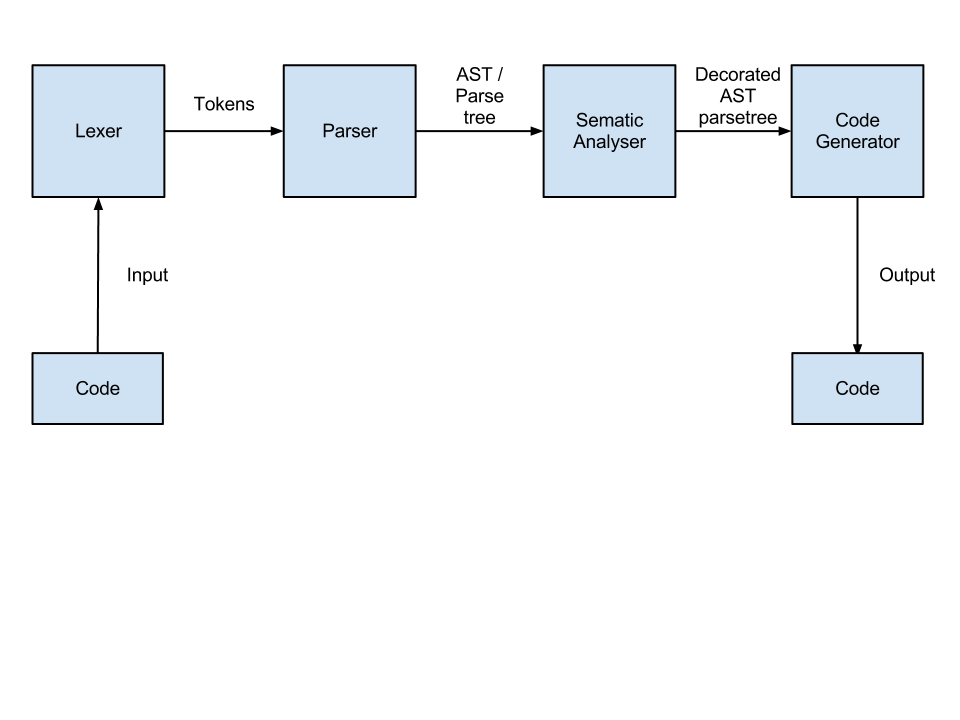
\includegraphics[width=250px]{images/Compilerconstruction.png}
		 \caption{Compiler construction}
	\label{fig:Compilerconstruction}
\end{figure}
